
\begin{figure}[h]
\centering
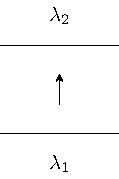
\includegraphics{fig_lambda_1_lambda_2.pdf}
\caption{Partition function between two boundary states of $S_i( \theta_1)$ and that of $S_j( \theta_2 )$}
\label{fig:fig_lambda_1_lambda_2}
\end{figure}

In this appendix, we calculate the amplitude between general boundary states defined in Eq.~\eqref{eq:Zab-bd}
\begin{equation}
\begin{aligned}
Z_{ab} &= \langle 0 | \exp\Big\{  \vec{b} R_b( \theta )    \vec{\bar{b}} \Big\}  \exp\Big\{ -\vec{b}^{\dagger}  (\mathbb{I}_2  \otimes M)  \vec{b} \Big\} \\
&\exp\Big\{  \vec{b}^{\dagger} R_a( \theta )    \vec{\bar{b}}^{\dagger} \Big\} | 0\rangle,
\end{aligned}
\end{equation}
where
\begin{equation}
\begin{aligned}
M &=  \frac{4\pi^2}{\beta} \text{diag}( 1, 2, \cdots ), \quad  \mathbb{I}_2 = \text{diag}( 1, 1), \\
R_i &= S_i( \theta ) \otimes \mathbb{I}.
\end{aligned}
\end{equation}
Using the identity Eq.~\eqref{eq:second_id_in_app_pf_of_id} proven in App.~\ref{app:pf_of_id}, we have
\begin{equation}
Z_{ab} = \frac{1}{\det(1 - R_a^{\dagger} e^{- \mathbb{I}_2 \otimes M} R_b )}
\end{equation}
From $|\det( R_a R_b^{\dagger})|  = 1$, free energy becomes
\begin{equation}
F = - \ln |Z_{ab}| = \ln |\det ( R_a R_b^{\dagger} - e^{- \mathbb{I}_2 \otimes M} )| .
\end{equation}
There are two cases to be considered, and we only take out the leading order term in $\beta$. 
\begin{itemize}
\item {\it case 1: }$S_1( \theta_1 ) \rightarrow S_2 ( \theta_2 ) $, the free energy is
\begin{equation}
\begin{aligned}
F & = \ln |\det ( R_1( \theta_1 )  R_2^{\dagger}( \theta_2 )  - e^{- \mathbb{I}_2 \otimes M} )| \\
  & = \ln \left| \det
\begin{bmatrix}
-\cos 2 \Delta \theta \mathbb{I} - e^{-M}   & -\sin 2 \Delta \theta \mathbb{I}\\
- \sin 2\Delta \theta \mathbb{I}  &   \cos 2 \Delta \theta \mathbb{I} - e^{-M} \\ 
\end{bmatrix} \right| \\
& = \sum_i \ln [ 1 -  e^{- 2 \lambda_i }  ] \\
& = \frac{\beta}{4\pi^2} \int_0^{\infty} dx \ln [ 1 - e^{-2x} ]  = - \frac{1}{48 }\beta .
\end{aligned}
\end{equation}
\item {\it case 2:} $S_i( \theta_1 ) \rightarrow S_i( \theta_2 )$, where $i = 1 $ or $ 2$, 
\begin{equation}
\begin{aligned}
F & = \ln \det 
\begin{bmatrix}
\cos 2 \Delta \theta \mathbb{I} - e^{-M}   & \sin 2 \Delta \theta \mathbb{I}\\
- \sin 2\Delta \theta \mathbb{I}  &   \cos 2 \Delta \theta \mathbb{I} - e^{-M} \\ 
\end{bmatrix} \\
& = \sum_i \ln [ 1 - 2 \cos 2 \Delta \theta e^{- \lambda_i } + e^{- 2 \lambda_i }  ] \\
& = \frac{\beta}{4\pi^2} \int_0^{\infty} dx \ln [ 1 - 2 \cos 2 \Delta \theta e^{-x} + e^{-2x} ] ,
\end{aligned}
\end{equation}
where $\Delta \theta = \theta_2 - \theta_1$. This integral is an even function of $\Delta \theta$ and the $\Delta \theta > 0$ case reduce to the polylog and Bernoulli polynomial
\begin{equation}
\begin{aligned}
  F &= \frac{\beta}{4\pi^2} \left[ - \text{Li}_2 ( e^{2i |\Delta \theta|} ) - \text{Li}_2 ( e^{- 2i |\Delta \theta|} ) \right] \\
  & = \frac{\beta}{4\pi^2}  \left[ - 2\pi^2 B_2 (|x|) \right] \\
  &= - \frac{\beta}{2} B_2( |x| )  = \frac{\beta}{2} (| x| - x^2 - \frac{1}{6} ),
\end{aligned}
\end{equation}
where $x = \frac{\Delta \theta}{ \pi}$. 
\end{itemize}




%%% Local Variables:
%%% TeX-master: "bCFT_paper"
%%% TeX-PDF-mode: t
%%% End:
